\mychapter{Procedimento Experimental}
\label{Cap:Procedimento}

Esse capítulo descreve os dispositivos e a metodologia utilizada na execução dos experimentos, o cenário onde esses experimentos formam realizados e, por fim, os experimentos realizados para aferir parâmetros de funcionamento dos módulos XBee PRO S3B 900HP.

\section{Tecnologias Utilizadas}

Além do módulo XBee PRO S3B 900HP (fig \ref{fig:xbeepro}), foram utilizados na execução dos experimentos: módulos \emph{XBee Explorer}, aeronaves \emph{Phantom 3 Standard}, o \emph{software} XCTU utilizado para a realização dos testes e uma fonte de alimentação externa para alimentar o conjunto módulo XBee + XBee \emph{Explorer}.

As especificações técnicas, bem como o modo de funcionamento, dos módulos XBee já foram discutidos no capítulo \ref{Cap:Xbee}. Os demais materiais utilizados serão descritos a seguir.

\begin{figure}[h!] 
\center
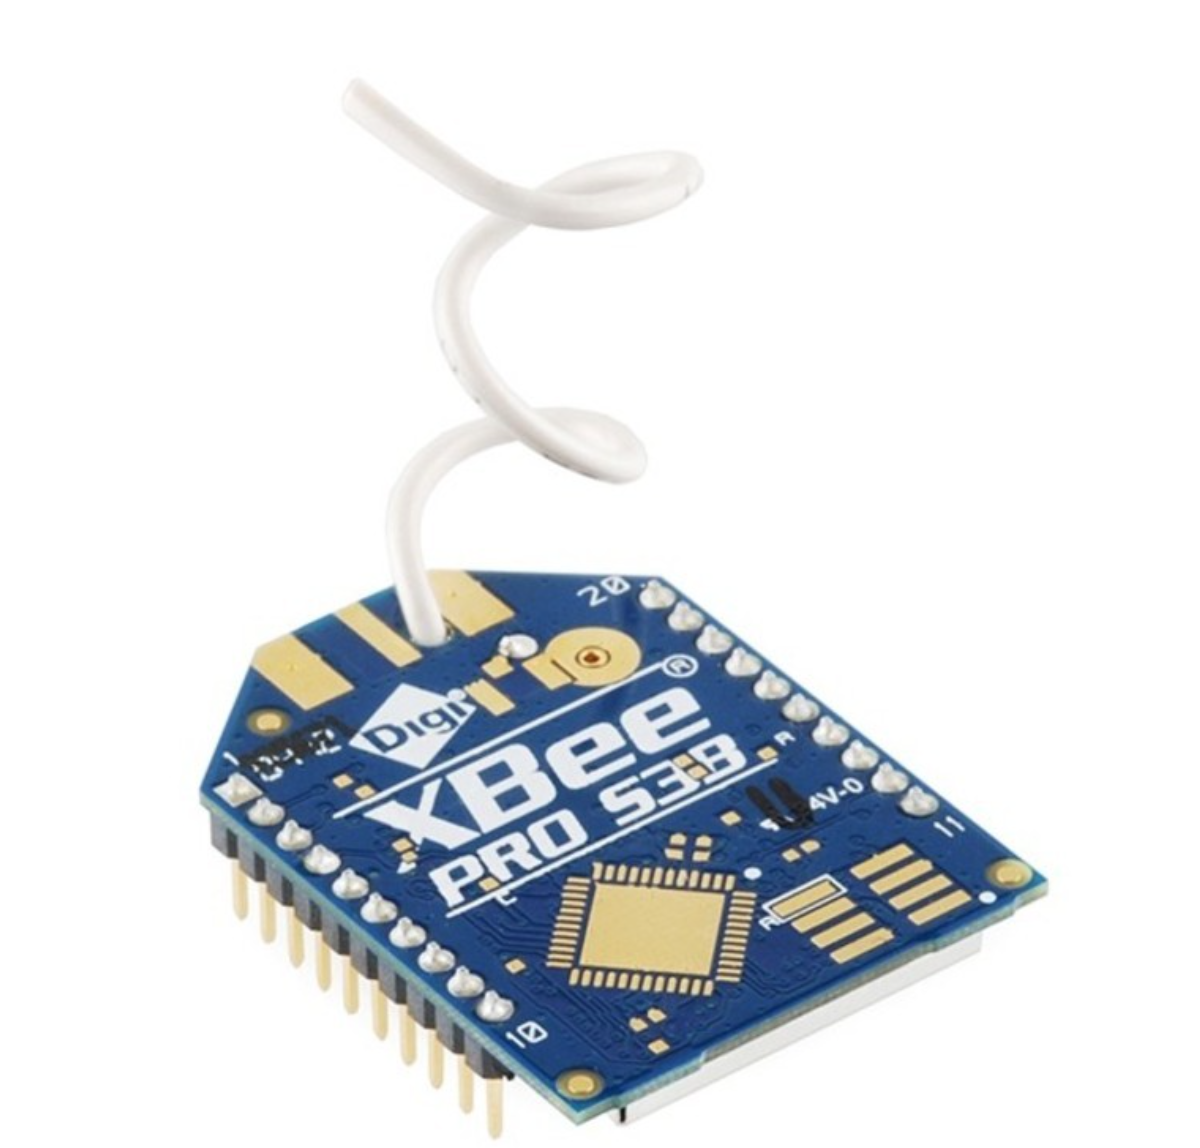
\includegraphics[width=0.7\textwidth]{xbeepro.png}
\caption{Módulo XBee PRO S3B 900HP.} 
\label{fig:xbeepro}
\end{figure}

\subsection{XBee Explorer}

O XBee \emph{Explorer} é a \emph{interface} de \emph{hardware} utilizada para conectar um módulo XBee a outros dispositivos, como por exemplo um computador. O módulo adquirido pelo projeto, como mostra a figura \ref{fig:xbeeexplorer}, possui duas formas de acesso ao módulo XBee acoplado a ele, sendo essas uma porta micro usb, utilizada para alimentação e comunicação, ou um conjunto de pinos contendo Rx, Tx, \emph{reset} e os pinos a serem utilizados para alimentação.

Apesar de da voltagem de alimentação dos módulos XBee ser de +3.3 volts, o XBee \emph{Explorer} deve ser alimentado com uma fonte que forneça +5 volts, que é reduzida para a voltagem de alimentação requerida pelo módulo XBee através da circuitaria do \emph{Explorer}.

\begin{figure}[h!] 
\center
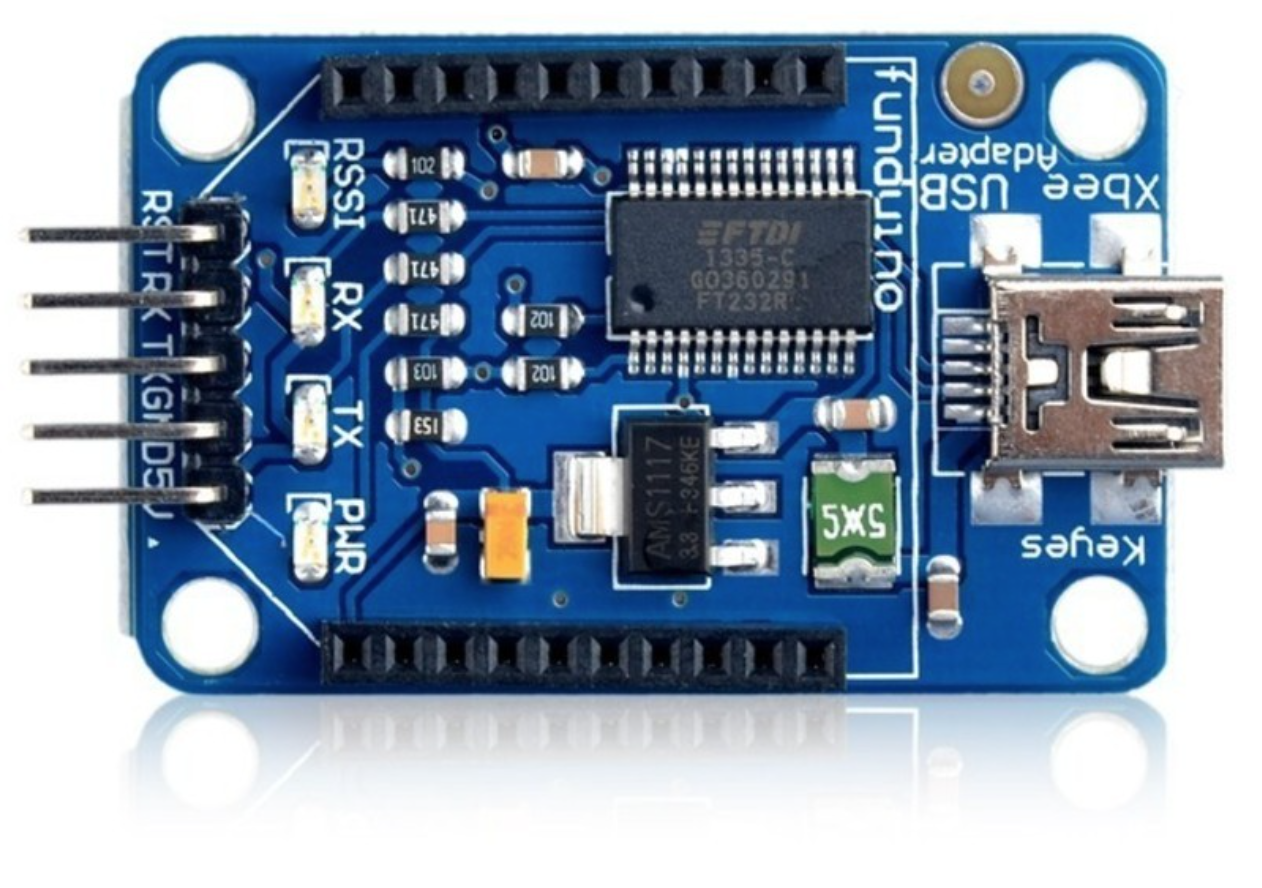
\includegraphics[width=0.7\textwidth]{xbeeexplorer.png}
\caption{XBee Explorer.} 
\label{fig:xbeeexplorer}
\end{figure} 

\subsection{Phantom 3 Standard}

Outro dispositivo de grande importância para a realização dos experimentos foram os quadrirrotores do modelo \emph{Phantom 3 Standard} (figura \ref{fig:phantom}) adquiridos pelo projeto e utilizados para variação e medição da distância entre os nós da rede \emph{mesh} formada para a realização dos teste de performance.

A escolha desse modelo de quadrirrotor se deu pela facilidade de voo e manutenção das aeronaves e os modos de voo personalizados, em especial a função de voo em trajetória circular em torno de um ponto fixo com velocidade controlada. Nesse modo de voo o operador da aeronave define o centro da trajetória circular, o raio e a velocidade a qual a aeronave vai voar. Como discutido nas próximas sessões, esse modo de voo foi utilizado nos experimentos realizados para medir o efeito da movimentação dos nós da rede na qualidade do \emph{link}, consequentemente, da rede multi VANT.

\begin{figure}[h!] 
\center
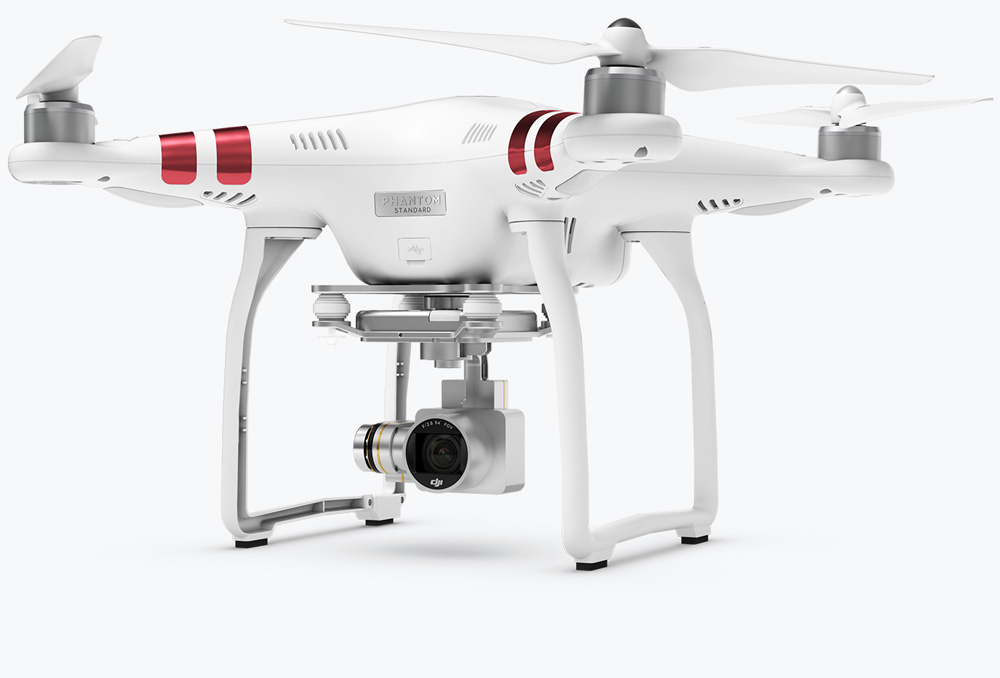
\includegraphics[width=0.7\textwidth]{phatom.jpg}
\caption{Aeronave Phantom 3 \emph{Standard}.} 
\label{fig:phantom}
\end{figure}

\subsection{XCTU}

O XCTU, bevemente apresentado no capítulo \ref{Cap:Xbee}, é o \emph{software}, disponibilizado pela fabricante dos módulos XBee, utilizado para configuração dos dispositivos e que também possui algumas ferramentas para analise da qualidade da rede formada. Ferramentas essas que foram utilizadas nesse trabalho para aferir a qualidade da rede, em especial o teste de força de sinal e o de taxa de transmissão (\emph{throughput}).

As figuras \ref{fig:rangeTest} e \ref{fig:throughput} apresentam, respectivamente, as telas dos testes de força de sinal e taxa de transmissão disponíveis no \emph{software} XCTU.

\begin{figure}[h!] 
\center
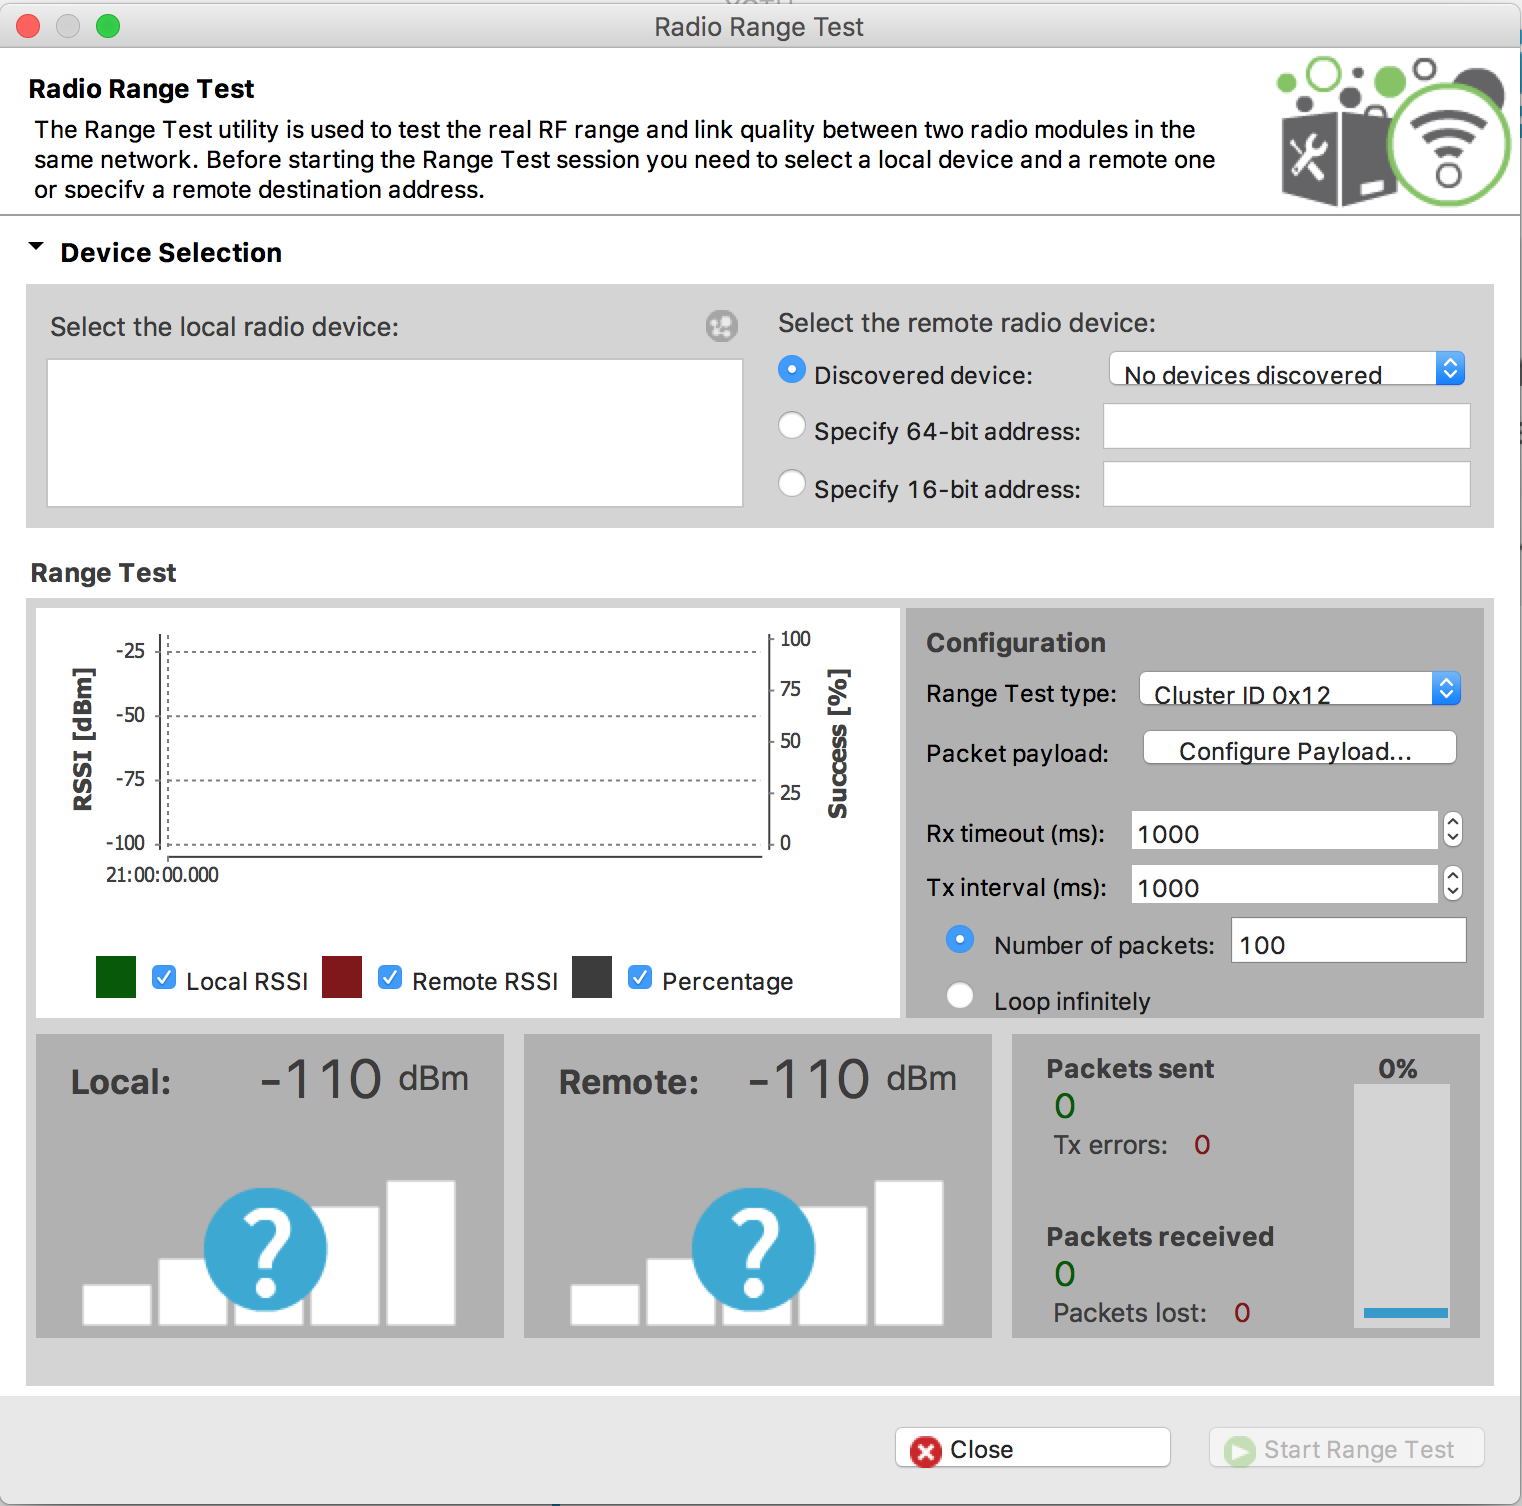
\includegraphics[width=0.7\textwidth]{RangeTest.png}
\caption{Tela do teste de força de sinal.} 
\label{fig:rangeTest}
\end{figure}

\begin{figure}[h!] 
\center
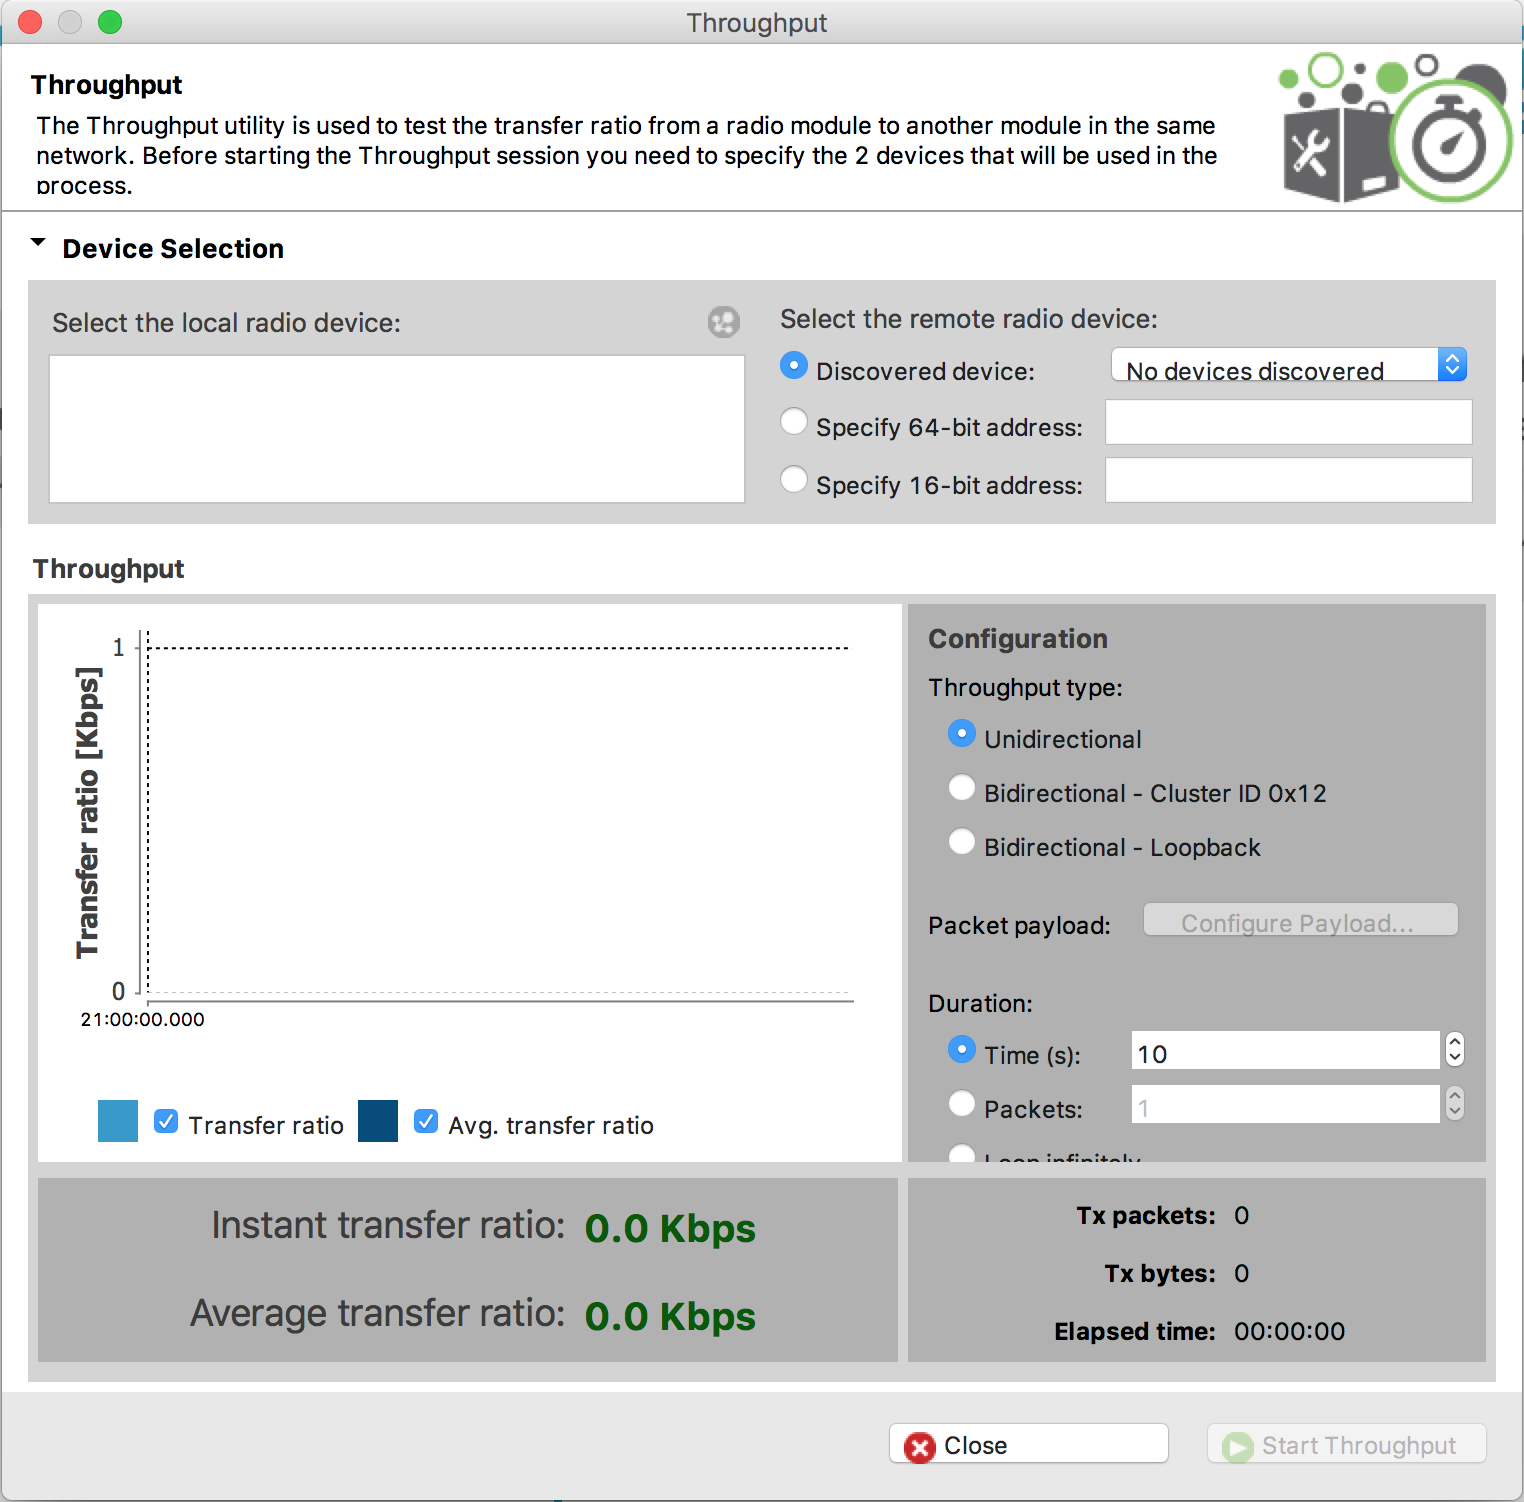
\includegraphics[width=0.7\textwidth]{ThroughputTest.png}
\caption{Tela do teste de taxa de transmissão (\emph{throughput}).} 
\label{fig:throughput}
\end{figure}

\section{Local dos Experimentos}

O local ideal para a realização dos experimentos seria o local onde o sistema final seria utilizado, ou seja, o próprio Centro de Lançamento Barreira do Inferno (CLBI), pois os testes refletiriam as condições especificas de interferência e meio de comunicação onde a rede multi VANTs será operada.

Infelizmente, devido a indisponibilidade de tempo e acesso, os testes de campo aqui apresentados foram realizados em sua maioria no campo central da Universidade Federal do Rio Grande do Norte (UFRN), o que pode ser considerado um ambiente urbano e pode apresentar níveis de interferência de sinal maiores que o ambiente onde a rede será de fato operacionalizada. Ja os testes de bancada forma realizados no laboratório de robótica localizado no Departamento de Computação e Automação (DCA).

\section{Experimentos Realizados}

No intuito de aferir a qualidade dos \emph{links} e, consequentemente, a rede a qual eles fazem parte, no contexto de um rede multi VANTs, foram realizados múltiplos testes de força de sinal e taxa de transmissão para diferente cenários, sendo eles:

\begin{itemize}
\item Teste de bancada
\item Teste em ar com posição fixa
\item Teste em ar em trajetória circular
\end{itemize} 

\subsection{Teste de Bancada}



\subsection{Teste em Ar com Posição Fixa}



\subsection{Teste em Ar em Trajetória Circular}
